\section{Introduzione}
\subsection{Scopo del prodotto}
Lo scopo è quello di fornire uno strumento intuitivo e immersivo per gli utenti che voglio partecipare all'esperienza di esplorare un acquario con i suoi ornamenti e decorazioni.
\newline
Le decorazioni vengono così esposte e visualizzate in un modo molto più autentico e coinvolgente.

\subsection{Descrizione generale}
Per rendere il documento il più esauriente possibile ma allo stesso tempo non troppo prolisso, abbiamo schematizzato ogni caso d'uso evidenziando:  precondizioni, postcondizioni, scenario principale in cui tale azione avrà luogo, una breve descrizione ed eventuali estensioni.\newline
In alcuni casi è stata anche inserita un'immagine dello schema UML per fornire una spiegazione visiva che può aiutare nel comprendere più a fondo il nostro lavoro.\newline
Da notare, nelle immagini dello schema UML sono stati rappresentati in azzurro i casi d'uso facoltativi.

\subsection{Attori}
Data l'ampiezza e struttura ridotta del software, l'attore che interagisce col nostro software è uno solo, denominato "Utente in ambiente 3D". 

\subsubsection{Utente in ambiente 3D}
Si tratta dell'utente protagonista di tutti i casi d'uso del nostro prodotto, chiamato tale dato che il software fornisce un immersione completa all'interno dello scenario 3D. \newline
L'utente non verrai mai reindirizzato a una normale pagina web statica, poiché ne risentirebbe la user experience. 

\pagebreak

\section{Casi d'uso}

\subsection{UC 1 - Rimozione oggetto singolo dal carrello}

\begin{itemize}
	
	\item Attore primario: 
	\begin{itemize}
		\item Utente in ambiente 3D.
	\end{itemize}
	\item Descrizione:
	\begin{itemize}
		\item Viene rimosso un singolo oggetto dal carrello.
	\end{itemize}
	
	\item Precondizioni:
	\begin{itemize}
		\item Il carrello contiene almeno un oggetto.
	\end{itemize}
	
	\item Postcondizioni:
	\begin{itemize}
		\item Un oggetto è stato rimosso dal carrello.
	\end{itemize}
	
	\item Scenario principale:
	\begin{itemize}
		\item L'utente interagisce con il sistema per la rimozione di un oggetto dal carrello.
	\end{itemize}
	
\end{itemize}

\pagebreak

\subsection{UC 2 - Svuotamento totale carrello}
\begin{itemize}
	
	\item Attore primario: 
	\begin{itemize}
		\item Utente in ambiente 3D.
	\end{itemize}
	\item Descrizione:
	\begin{itemize}
		\item Prevede la rimozione di tutti gli oggetti presenti nel carrello con un singolo comando.
	\end{itemize}
	
	\item Precondizioni:
	\begin{itemize}
		\item Il carrello contiene almeno un oggetto.
	\end{itemize}
	
	\item Postcondizioni:
	\begin{itemize}
		\item Tutti gli oggetti sono stati rimossi dal carrello;
		\item Il carrello è vuoto.
	\end{itemize}
	
	\item Scenario principale:
	\begin{itemize}
		\item L'utente interagisce con il sistema per svuotare completamente il carrello.
	\end{itemize}
	
\end{itemize}

\pagebreak

\subsection{UC 3 - Visualizzazione contenuto del carrello}

\begin{figure}[H]
  \renewcommand{\thefigure}{1}
  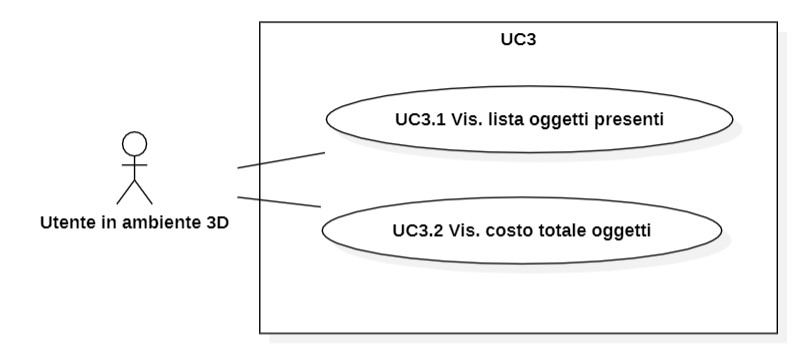
\includegraphics[width=\linewidth]{./res/images/UC3.png}
  \caption{UC 3 - Visualizzazione contenuto del carrello}
  \label{fig:UC 3}
\end{figure}

\begin{itemize}
	
	\item Attore primario: 
	\begin{itemize}
		\item Utente in ambiente 3D.
	\end{itemize}
	\item Descrizione:
	\begin{itemize}
		\item Permette di visualizzare il contenuto del carrello.
	\end{itemize}
	
	\item Precondizioni:
	\begin{itemize}
		\item Il contenuto del carrello è nascosto.
	\end{itemize}
	
	\item Postcondizioni:
	\begin{itemize}
		\item Il contenuto del carrello è visibile.
	\end{itemize}
	
	\item Scenario principale:
	\begin{itemize}
		\item L'utente interagisce con il sistema per visualizzare il contenuto del carrello.
	\end{itemize}
	
\end{itemize}

\subsubsection{UC 3.1 - Visualizzazione oggetti presenti}

\begin{figure}[H]
  \renewcommand{\thefigure}{2}
  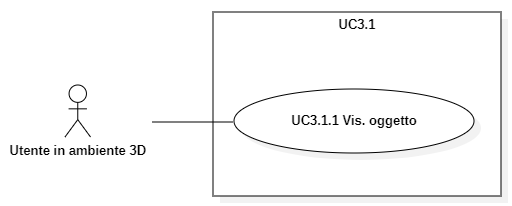
\includegraphics[width=\linewidth]{./res/images/UC3.1.png}
  \caption{UC 3.1 - Visualizzazione oggetti presenti con relative caratteristiche e quantità}
  \label{fig:UC 3.1}
\end{figure}

\begin{itemize}
	
	\item Attore primario: 
	\begin{itemize}
		\item Utente in ambiente 3D.
	\end{itemize}
	\item Descrizione:
	\begin{itemize}
		\item L'utente può visualizzare la lista degli oggetti presenti nel carrello.
	\end{itemize}
	
	\item Precondizioni:
	\begin{itemize}
		\item Il contenuto del carrello è visibile.
	\end{itemize}
	
	\item Postcondizioni:
	\begin{itemize}
		\item Il contenuto del carrello è visibile;
		\item La lista degli oggetti presenti all'interno del carrello è visibile.
	\end{itemize}
	
	\item Scenario principale:
	\begin{itemize}
		\item Nessuna azione richiesta.
	\end{itemize}
	
\end{itemize}

\paragraph{UC 3.1.1 - Visualizzazione oggetto}

\begin{figure}[H]
  \renewcommand{\thefigure}{3}
  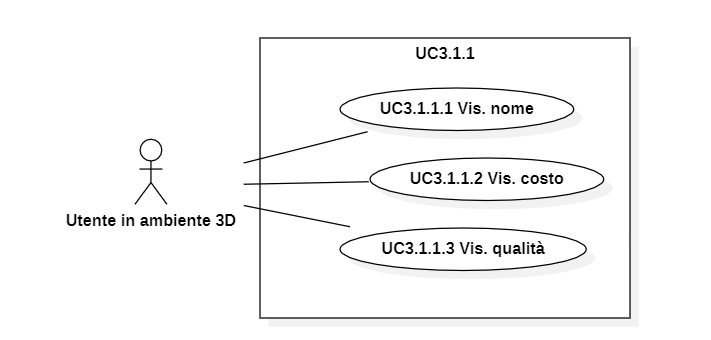
\includegraphics[width=\linewidth]{./res/images/UC3.1.1.png}
  \caption{UC 3.1.1 - Visualizzazione oggetto}
  \label{fig:UC 3.1.1}
\end{figure}

\begin{itemize}
	
	\item Attore primario: 
	\begin{itemize}
		\item Utente in ambiente 3D.
	\end{itemize}
	\item Descrizione:
	\begin{itemize}
		\item Prevede la visualizzazione la visualizzazione di un oggetto all'interno della lista oggetti del carrello.
	\end{itemize}
	
	\item Precondizioni:
	\begin{itemize}
		\item La lista degli oggetti presenti all'interno del carrello è visibile.
	\end{itemize}
	
	\item Postcondizioni:
	\begin{itemize}
		\item La lista degli oggetti presenti all'interno del carrello è visibile;
		\item L'oggetto è visibile nella lista oggetti del carrello.
	\end{itemize}
	
	\item Scenario principale:
	\begin{itemize}
		\item Nessuna azione richiesta.
	\end{itemize}
	
\end{itemize}

\subparagraph{UC 3.1.1.1 - Visualizzazione nome}
\begin{itemize}
	
	\item Attore primario: 
	\begin{itemize}
		\item Utente in ambiente 3D.
	\end{itemize}
	\item Descrizione:
	\begin{itemize}
		\item Prevede la visualizzazione del nome dell'oggetto, il nome dell'oggetto è un identificativo che permette di distinguere oggetti diversi tra loro.
	\end{itemize}
	
	\item Precondizioni:
	\begin{itemize}
		\item L'oggetto è visibile nella lista oggetti del carrello.
	\end{itemize}
	
	\item Postcondizioni:
	\begin{itemize}
		\item L'oggetto è visibile nella lista oggetti del carrello;
		\item Il nome associato all'oggetto è visibile.
	\end{itemize}
	
	\item Scenario principale:
	\begin{itemize}
		\item Nessuna azione richiesta.
	\end{itemize}
	
\end{itemize}

\subparagraph{UC 3.1.1.2 - Visualizzazione costo}
\begin{itemize}
	
	\item Attore primario: 
	\begin{itemize}
		\item Utente in ambiente 3D.
	\end{itemize}
	\item Descrizione:
	\begin{itemize}
		\item Prevede la visualizzazione del costo dell'oggetto.
	\end{itemize}
	
	\item Precondizioni:
	\begin{itemize}
		\item L'oggetto è visibile nella lista oggetti del carrello.
	\end{itemize}
	
	\item Postcondizioni:
	\begin{itemize}
		\item L'oggetto è visibile nella lista oggetti del carrello;
		\item Il costo associato all'oggetto è visibile.
	\end{itemize}
	
	\item Scenario principale:
	\begin{itemize}
		\item Nessuna azione richiesta.
	\end{itemize}
	
\end{itemize}

\subparagraph{UC 3.1.1.3 - Visualizzazione quantità}
\begin{itemize}
	
	\item Attore primario: 
	\begin{itemize}
		\item Utente in ambiente 3D.
	\end{itemize}
	\item Descrizione:
	\begin{itemize}
		\item Prevede la visualizzazione del numero di oggetti identici all'oggetto (compreso) presenti all'interno del carrello.
	\end{itemize}
	
	\item Precondizioni:
	\begin{itemize}
		\item L'oggetto è visibile nella lista oggetti del carrello.
	\end{itemize}
	
	\item Postcondizioni:
	\begin{itemize}
		\item L'oggetto è visibile nella lista oggetti del carrello;
		\item La quantità di oggetti identici all'oggetto (compreso) è visibile.
	\end{itemize}
	
	\item Scenario principale:
	\begin{itemize}
		\item Nessuna azione richiesta.
	\end{itemize}
	
\end{itemize}

\subsubsection{UC 3.2 - Visualizzazione costo totale oggetti}
\begin{itemize}
	
	\item Attore primario: 
	\begin{itemize}
		\item Utente in ambiente 3D.
	\end{itemize}
	\item Descrizione:
	\begin{itemize}
		\item Prevede la visualizzazione della somma di tutti i costi degli oggetti presenti all'interno del carrello.
	\end{itemize}
	
	\item Precondizioni:
	\begin{itemize}
		\item Il contenuto del carrello è visibile.
	\end{itemize}
	
	\item Postcondizioni:
	\begin{itemize}
		\item Il contenuto del carrello è visibile;
		\item Il totale della somma di tutti i costi degli oggetti presenti nel carrello è visibile.
	\end{itemize}
	
	\item Scenario principale:
	\begin{itemize}
		\item Nessuna azione richiesta.
	\end{itemize}
	
\end{itemize}

\pagebreak

\subsection{UC 4 - Aggiungere un oggetto al carrello}
\begin{itemize}

	\item Attore primario: 
	\begin{itemize}
		\item Utente in ambiente 3D.
	\end{itemize}
	\item Descrizione:
	\begin{itemize}
		\item Aggiungere un oggetto al carrello significa aggiungere alla lista degli oggetti presenti nel carrello l'oggetto desiderato e visualizzare un messaggio di oggetto aggiunto al carrello con successo.
\newline L'oggetto all'interno dell'ambiente continua ad esistere anche dopo la sua aggiunta al carrello.
	\end{itemize}
	
	\item Precondizioni:
	\begin{itemize}
		\item L'oggetto da aggiungere al carrello si trova all'interno dell'ambiente 3D.
	\end{itemize}
	
	\item Postcondizioni:
	\begin{itemize}
		\item L'oggetto aggiunto al carrello si trova all'interno dell'ambiente 3D;
		\item L'oggetto e' presente all'interno del carrello.
	\end{itemize}
	
	\item Scenario principale:
	\begin{itemize}
		\item L'utente interagisce con l'oggetto da aggiungere all'interno del carrello;
		\item L'utente seleziona il comando aggiungi oggetto al carrello.
	\end{itemize}
	
\end{itemize}

\pagebreak

\subsection{UC 5 - Compiere movimenti direzionali}

\begin{figure}[H]
  \renewcommand{\thefigure}{4}
  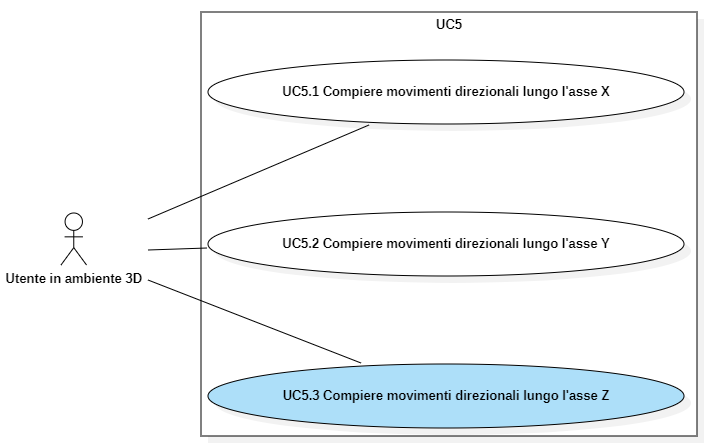
\includegraphics[width=\linewidth]{./res/images/UC5.png}
  \caption{UC 5 - Compiere movimenti direzionali}
  \label{fig:UC 5}
\end{figure}

\begin{itemize}

	\item Attore primario: 
	\begin{itemize}
		\item Utente in ambiente 3D.
	\end{itemize}
	\item Descrizione:
	\begin{itemize}
		\item Compiere azioni di movimenti direzionali significa interagire con il sistema per spostarsi nello spazio offerto dall'ambiente 3D.
	\end{itemize}
	
	\item Precondizioni:
	\begin{itemize}
		\item Le azioni di movimento direzionali devono essere abilitate;
		\item Le azioni di movimento direzionali devono essere valide;
		\item L'utente si trova in una posizione iniziale nello spazio.
	\end{itemize}
	
	\item Postcondizioni:
	\begin{itemize}
		\item L'utente si trova in una posizione diversa da quella iniziale nello spazio.
	\end{itemize}
	
	\item Scenario principale:
	\begin{itemize}
		\item L'utente interagisce con il sistema per compiere un'azione di movimento direzionale.
	\end{itemize}
	
\end{itemize}


\subsubsection{UC 5.1 - Compiere movimenti direzionali lungo l'asse X}
\begin{itemize}

	\item Attore primario: 
	\begin{itemize}
		\item Utente in ambiente 3D.
	\end{itemize}
	\item Descrizione:
	\begin{itemize}
		\item Caso d'uso autoesplicativo.
	\end{itemize}
	
	\item Precondizioni:
	\begin{itemize}
		\item Le azioni di movimento direzionale lungo l'asse delle X devono essere abilitate;
		\item Le azioni di movimento direzionali lungo l'asse X devono essere valide;
		\item L'utente si trova in una posizione iniziale nello spazio rispetto all'asse X.
	\end{itemize}
	
	\item Postcondizioni:
	\begin{itemize}
		\item L'utente si trova in una posizione diversa da quella iniziale nello spazio rispetto all'asse X.
	\end{itemize}
	
	\item Scenario principale:
	\begin{itemize}
		\item L'utente interagisce con il sistema per compiere un'azione di movimento direzionale lungo l'asse X.
	\end{itemize}
	
\end{itemize}

\subsubsection{UC 5.2 - Compiere movimenti direzionali lungo l'asse Y}
\begin{itemize}

	\item Attore primario: 
	\begin{itemize}
		\item Utente in ambiente 3D.
	\end{itemize}
	\item Descrizione:
	\begin{itemize}
		\item Caso d'uso autoesplicativo.
	\end{itemize}
	
	\item Precondizioni:
	\begin{itemize}
		\item Le azioni di movimento direzionale lungo l'asse delle Y devono essere abilitate;
		\item Le azioni di movimento direzionali lungo l'asse Y devono essere valide;
		\item L'utente si trova in una posizione iniziale nello spazio rispetto all'asse Y.
	\end{itemize}
	
	\item Postcondizioni:
	\begin{itemize}
		\item L'utente si trova in una posizione diversa da quella iniziale nello spazio rispetto all'asse Y.
	\end{itemize}
	
	\item Scenario principale:
	\begin{itemize}
		\item L'utente interagisce con il sistema per compiere un'azione di movimento direzionale lungo l'asse Y.
	\end{itemize}
	
\end{itemize}

\subsubsection{UC 5.3 - Compiere movimenti direzionali lungo l'asse Z}
\begin{itemize}

	\item Attore primario: 
	\begin{itemize}
		\item Utente in ambiente 3D.
	\end{itemize}
	\item Descrizione:
	\begin{itemize}
		\item Caso d'uso autoesplicativo.
	\end{itemize}
	
	\item Precondizioni:
	\begin{itemize}
		\item Le azioni di movimento direzionale lungo l'asse delle Z devono essere abilitate;
		\item Le azioni di movimento direzionali lungo l'asse Z devono essere valide;
		\item L'utente si trova in una posizione iniziale nello spazio rispetto all'asse Z.
	\end{itemize}
	
	\item Postcondizioni:
	\begin{itemize}
		\item L'utente si trova in una posizione diversa da quella iniziale nello spazio rispetto all'asse Z.
	\end{itemize}
	
	\item Scenario principale:
	\begin{itemize}
		\item L'utente interagisce con il sistema per compiere un'azione di movimento direzionale lungo l'asse Z.
	\end{itemize}
	
\end{itemize}

\pagebreak

\subsection{UC 6 - Compiere rotazioni camera}
\begin{itemize}

	\item Attore primario: 
	\begin{itemize}
		\item Utente in ambiente 3D.
	\end{itemize}
	\item Descrizione:
	\begin{itemize}
		\item Compiere un'azione di spostamento camera permette all'utente di vedere l'ambiente che lo circonda variando la direzione della propria visuale.
	\end{itemize}
	
	\item Precondizioni:
	\begin{itemize}
		\item L'azione di spostamento camera deve essere abilitata;
		\item La visuale dell'utente è direzionata verso un punto iniziale.
	\end{itemize}
	
	\item Postcondizioni:
	\begin{itemize}
		\item La visuale dell'utente è direzionata verso un punto diverso rispetto a quello iniziale.
	\end{itemize}
	
	\item Scenario principale:
	\begin{itemize}
		\item L'utente interagisce con il sistema per compiere un'azione di spostamento camera.
	\end{itemize}
	
\end{itemize}

\pagebreak

\subsection{UC 7 - Modificare attributi oggetto}
\begin{itemize}

	\item Attore primario: 
	\begin{itemize}
		\item Utente in ambiente 3D.
	\end{itemize}
	\item Descrizione:
	\begin{itemize}
		\item Modificare attributi oggetto prevede la modifica degli attributi dell'oggetto che l'utente desidera modificare.
\newline A seconda dell'oggetto da modificare gli attributi modificabili potrebbero essere diversi.
\newline Potrebbero essere presenti anche oggetti non modificabili.
	\end{itemize}
	
	\item Precondizioni:
	\begin{itemize}
		\item L'oggetto da modificare si trova all'interno dell'ambiente 3D.
	\end{itemize}
	
	\item Postcondizioni:
	\begin{itemize}
		\item L'oggetto modificato si trova all'interno dell'ambiente 3D;
		\item L'oggetto è stato modificato;
		\item L'oggetto assume le caratteristiche visive dovute alle. modifiche
	\end{itemize}
	
	\item Scenario principale:
	\begin{itemize}
		\item L'utente interagisce con l'oggetto da modificare;
		\item L'utente seleziona il comando modifica oggetto;
		\item L'utente apporta le modifiche desiderate;
		\item L'utente conferma le modifiche.
	\end{itemize}
	
	\item Estensioni:
	\begin{itemize}
		\item UC 8 - Visualizzazione messaggio oggetto non modificabile.
	\end{itemize}
	
\end{itemize}

\pagebreak

\subsection{UC 8 - Visualizzazione messaggio oggetto non modificabile}
\begin{itemize}

	\item Attore primario: 
	\begin{itemize}
		\item Utente in ambiente 3D.
	\end{itemize}
	\item Descrizione:
	\begin{itemize}
		\item Prevede la visualizzazione di un messaggio informativo di "oggetto non modificabile".
\newline Un oggetto potrebbe non essere modificabile per la presenza di una sola configurazione per quell'oggetto.
	\end{itemize}
	
	\item Precondizioni:
	\begin{itemize}
		\item L'oggetto da modificare si trova all'interno dell'ambiente 3D;
		\item L'oggetto desiderato non è modificabile.
	\end{itemize}
	
	\item Postcondizioni:
	\begin{itemize}
		\item L'oggetto non è stato modificato;
		\item L'oggetto mantiene le sue caratteristiche visive.
	\end{itemize}
	
	\item Scenario principale:
	\begin{itemize}
		\item L'utente interagisce con l'oggetto da modificare;
		\item L'utente seleziona il comando modifica oggetto.
	\end{itemize}
	
\end{itemize}

\pagebreak

\subsection{UC 9 - Visualizzazione lista oggetti della stanza attuale}

\begin{figure}[H]
  \renewcommand{\thefigure}{5}
  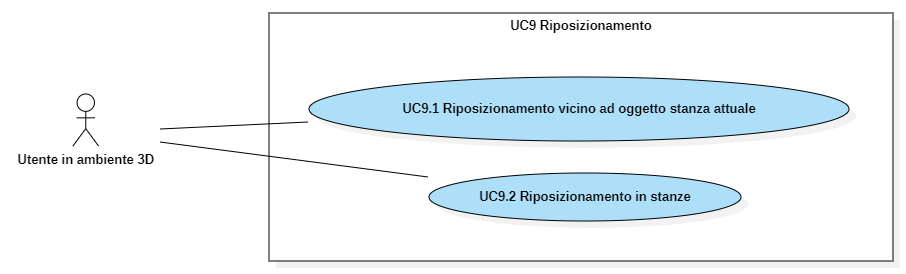
\includegraphics[width=\linewidth]{./res/images/UC9.png}
  \caption{UC 9 - Visualizzazione lista oggetti della stanza attuale}
  \label{fig:UC 9}
\end{figure}

\begin{itemize}

	\item Attore primario: 
	\begin{itemize}
		\item Utente in ambiente 3D.
	\end{itemize}
	\item Descrizione:
	\begin{itemize}
		\item Visualizza la lista di tutti gli oggetti presenti nella stanza.
	\end{itemize}
	
	\item Precondizioni:
	\begin{itemize}
		\item Il contenuto della lista oggetti è nascosto.
	\end{itemize}
	
	\item Postcondizioni:
	\begin{itemize}
		\item Il contenuto della lista oggetti è visibile.
	\end{itemize}
	
	\item Scenario principale:
	\begin{itemize}
		\item L'utente interagisce con il sistema per rendere il contenuto della lista oggetti visibile.
	\end{itemize}
	
\end{itemize}

\subsubsection{UC 9.1 - Visualizzazione nome oggetto nella lista}
\begin{itemize}

	\item Attore primario: 
	\begin{itemize}
		\item Utente in ambiente 3D.
	\end{itemize}
	\item Descrizione:
	\begin{itemize}
		\item Prevede la visualizzazione del nome dell’oggetto, il nome dell’oggetto `e un identificativo che permette di distinguere oggetti diversi tra loro.
	\end{itemize}
	
	\item Precondizioni:
	\begin{itemize}
		\item Il contenuto della lista oggetti è visibile.
	\end{itemize}
	
	\item Postcondizioni:
	\begin{itemize}
		\item Il nome dell'oggetto è visibile.
	\end{itemize}
	
	\item Scenario principale:
	\begin{itemize}
		\item Nessuna azione richiesta.
	\end{itemize}
	
\end{itemize}

\pagebreak

\subsection{UC 10 - Visualizzazione dettagli oggetto nel carrello}

\begin{figure}[H]
  \renewcommand{\thefigure}{6}
  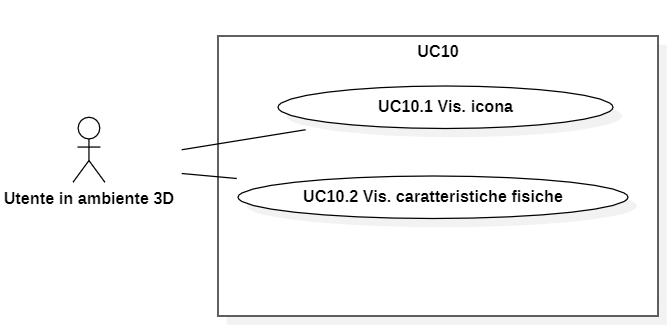
\includegraphics[width=\linewidth]{./res/images/UC10.png}
  \caption{UC 10 - Visualizzazione dettagli oggetto nel carrello}
  \label{fig:UC 10}
\end{figure}

\begin{itemize}
	
	\item Attore primario: 
	\begin{itemize}
		\item Utente in ambiente 3D.
	\end{itemize}
	\item Descrizione:
	\begin{itemize}
		\item Selezionando un oggetto nel carrello, l'utente può visualizzarne i dettagli.
	\end{itemize}
	
	\item Precondizioni:
	\begin{itemize}
		\item L'oggetto è visibile nella lista oggetti del carrello.
	\end{itemize}
	
	\item Postcondizioni:
	\begin{itemize}
		\item Vengono visualizzati a schermo i dettagli dell'oggetto.
	\end{itemize}
	
	\item Scenario principale:
	\begin{itemize}
		\item L'utente in ambiente 3D seleziona un oggetto dalla lista.
	\end{itemize}
	
\end{itemize}

\subsubsection{UC 10.1 - Visualizzazione icona}
\begin{itemize}
	
	\item Attore primario: 
	\begin{itemize}
		\item Utente in ambiente 3D.
	\end{itemize}
	\item Descrizione:
	\begin{itemize}
		\item Prevede la visualizzazione di un'icona associata all'oggetto a cui fa riferimento, l'icona è un'anteprima miniaturizzata dell'oggetto a cui fa riferimento.
	\end{itemize}
	
	\item Precondizioni:
	\begin{itemize}
		\item L'oggetto è stato selezionato dal carrello.
	\end{itemize}
	
	\item Postcondizioni:
	\begin{itemize}
		\item L'icona associata all'oggetto è visibile.
	\end{itemize}
	
	\item Scenario principale:
	\begin{itemize}
		\item Nessuna azione richiesta.
	\end{itemize}
	
\end{itemize}


\subsubsection{UC 10.2 - Visualizzazione caratteristiche fisiche}
\begin{itemize}
	
	\item Attore primario: 
	\begin{itemize}
		\item Utente in ambiente 3D.
	\end{itemize}
	\item Descrizione:
	\begin{itemize}
		\item Prevede la visualizzazione delle caratteristiche fisiche dell'oggetto, le caratteristiche fisiche dipendono dall'oggetto.
	\end{itemize}
	
	\item Precondizioni:
	\begin{itemize}
		\item L'oggetto è stato selezionato dal carrello.
	\end{itemize}
	
	\item Postcondizioni:
	\begin{itemize}
		\item Le caratteristiche fisiche dell'oggetto sono visibili.
	\end{itemize}
	
	\item Scenario principale:
	\begin{itemize}
		\item Nessuna azione richiesta.
	\end{itemize}
	
\end{itemize}

\pagebreak

\subsection{UC 11 - Riposizionamento vicino ad oggetto stanza attuale}
\begin{itemize}

	\item Attore primario: 
	\begin{itemize}
		\item Utente in ambiente 3D.
	\end{itemize}
	\item Descrizione:
	\begin{itemize}
		\item Riposizionamento vicino ad oggetto stanza attuale prevede il riposizionamento dell'utente vicino ad un oggetto
della stanza in cui si trova.
	\end{itemize}
	
	\item Precondizioni:
	\begin{itemize}
		\item L'utente si trova in un punto di partenza.
	\end{itemize}
	
	\item Postcondizioni:
	\begin{itemize}
		\item L'utente si trova nelle vicinanze dell'oggetto desiderato in un punto prestabilito.
	\end{itemize}
	
	\item Scenario principale:
	\begin{itemize}
		\item L'utente seleziona il comando per riposizionarsi nelle vicinanze di un oggetto.
	\end{itemize}
	
\end{itemize}

\pagebreak

\subsection{UC 12 - Riposizionamento in stanze}
\begin{itemize}

	\item Attore primario: 
	\begin{itemize}
		\item Utente in ambiente 3D.
	\end{itemize}
	\item Descrizione:
	\begin{itemize}
		\item Riposizionamento in stanze prevede il riposizionamento dell'utente in un punto prestabilito di una stanza da lui selezionata.
	\end{itemize}
	
	\item Precondizioni:
	\begin{itemize}
		\item L'utente si trova in un punto di partenza di una determinata stanza.
	\end{itemize}
	
	\item Postcondizioni:
	\begin{itemize}
		\item L'utente si trova in un punto prestabilito di una stanza da lui selezionata.
	\end{itemize}
	
	\item Scenario principale:
	\begin{itemize}
		\item L'utente seleziona il comando per riposizionarsi nella stanza. desiderata
	\end{itemize}
	
\end{itemize}

\pagebreak

\subsection{UC 13 - Visualizzazione messaggio riposizionamento in stanza non avvenuto}
\begin{itemize}

	\item Attore primario: 
	\begin{itemize}
		\item Utente in ambiente 3D.
	\end{itemize}
	\item Descrizione:
	\begin{itemize}
		\item Viene visualizzato un messaggio informativo di riposizionamento in stanza non avvenuto, dopo che l'utente, posizionato ad
una distanza dal punto iniziale della stanza inferiore a quella consentita per il compiersi dell'azione, tenta il ricollocamento in tale stanza.
	\end{itemize}
	
	\item Precondizioni:
	\begin{itemize}
		\item L'utente si trova ad una distanza dal punto di riposizionamento della stanza da lui selezionata entro la quale non è consentito il ricollocamento;
		\item L'utente interagisce con il comando di riposizionamento in quella destinazione.
	\end{itemize}
	
	\item Postcondizioni:
	\begin{itemize}
		\item Viene visualizzato un messaggio informativo riposizionamento in stanza non avvenuto;
		\item Il riposizionamento non è stato effettuato.
	\end{itemize}
	
	\item Scenario principale:
	\begin{itemize}
		\item Nessuna azione richiesta.
	\end{itemize}
	
\end{itemize}

\pagebreak

\subsection{UC 14 - Visualizzazione messaggio riposizionamento in prossimità dell'oggetto selezionato non avvenuto}
\begin{itemize}

	\item Attore primario: 
	\begin{itemize}
		\item Utente in ambiente 3D.
	\end{itemize}
	\item Descrizione:
	\begin{itemize}
		\item Viene visualizzato un messaggio informativo di riposizionamento in prossimità dell'oggetto non avvenuto, dopo che l'utente, posizionato ad
una distanza dall'oggetto inferiore a quella consentita per il compiersi dell'azione, tenta il ricollocamento in tale oggetto.
	\end{itemize}
	
	\item Precondizioni:
	\begin{itemize}
		\item L'utente si trova ad una distanza dall'oggetto da lui selezionato entro la quale non è consentito riposizionamento;
		\item L'utente interagisce con il comando di riposizionamento selezionando l'oggetto che si trova ad una distanza entro la quale non è consentito il ricollocamento.
	\end{itemize}
	
	\item Postcondizioni:
	\begin{itemize}
		\item Il riposizionamento non è avvenuto;
		\item Viene visualizzato un messaggio informativo di riposizionamento in prossimità dell'oggetto non avvenuto.
	\end{itemize}
	
	\item Scenario principale:
	\begin{itemize}
		\item Nessuna azione richiesta.
	\end{itemize}
	
\end{itemize}

\pagebreak

\subsection{UC 15 - Visualizzazione contenuto lista stanze}
\begin{itemize}

	\item Attore primario: 
	\begin{itemize}
		\item Utente in ambiente 3D.
	\end{itemize}
	\item Descrizione:
	\begin{itemize}
		\item Visualizzazione contenuto lista stanze permette di visualizzare il contenuto della lista stanze.
\newline Il contenuto della lista stanze prevede l'elenco delle stanze presenti all'interno dell'ambiente 3D.
	\end{itemize}
	
	\item Precondizioni:
	\begin{itemize}
		\item Il contenuto della lista stanze è nascosto.
	\end{itemize}
	
	\item Postcondizioni:
	\begin{itemize}
		\item Il contenuto della lista stanze è visibile.
	\end{itemize}
	
	\item Scenario principale:
	\begin{itemize}
		\item L'utente interagisce con il sistema per rendere il contenuto della lista stanze visibile.
	\end{itemize}
	
\end{itemize}

\pagebreak

\subsection{UC 16 - Spostamento oggetto}
\begin{itemize}

	\item Attore primario: 
	\begin{itemize}
		\item Utente in ambiente 3D.
	\end{itemize}
	\item Descrizione:
	\begin{itemize}
		\item Riposizionamento di un oggetto in un altro punto della stanza in cui ci si trova.
	\end{itemize}
	
	\item Precondizioni:
	\begin{itemize}
		\item L'oggetto da spostare si trova all'interno dell'ambiente 3D;
		\item L'oggetto si trova in una coordinata X, Y, Z di una stanza.
	\end{itemize}
	
	\item Postcondizioni:
	\begin{itemize}
		\item L'oggetto si trova in una coordinata X, Y, Z diversa da quella di partenza nella stessa stanza.
	\end{itemize}
	
	\item Scenario principale:
	\begin{itemize}
		\item L'utente interagisce con l'oggetto per poterlo spostare in un altra coordinata all'interno della stanza di partenza.
	\end{itemize}
	
	\item Estensioni:
	\begin{itemize}
		\item UC 13 - Oggetto non posizionato.
	\end{itemize}
	
\end{itemize}

\pagebreak

\subsection{UC 17 - Oggetto non posizionato}
\begin{itemize}

	\item Attore primario: 
	\begin{itemize}
		\item Utente in ambiente 3D.
	\end{itemize}
	\item Descrizione:
	\begin{itemize}
		\item Se l'utente cerca di posizionare un oggetto in una coordinata X, Y, Z non legittima, l'oggetto non viene posizionato.
	\end{itemize}
	
	\item Precondizioni:
	\begin{itemize}
		\item L'oggetto si trova in una coordinata X, Y, Z non valida;
		\item L'oggetto è in fase di spostamento.
	\end{itemize}
	
	\item Postcondizioni:
	\begin{itemize}
		\item L'oggetto è in fase di spostamento;
		\item L'oggetto non è stato posizionato.
	\end{itemize}
	
	\item Scenario principale:
	\begin{itemize}
		\item Nessuna azione richiesta.
	\end{itemize}
	
\end{itemize}

\pagebreak

\subsection{UC 18 - Torcia}
\begin{itemize}

	\item Attore primario: 
	\begin{itemize}
		\item Utente in ambiente 3D.
	\end{itemize}
	\item Descrizione:
	\begin{itemize}
		\item L'utente può utilizzare una torcia per illuminare parte dell'ambiente di fronte a lui. \newline La torcia si può trovare in due stati, accesa o spenta.
	\end{itemize}
	
	\item Precondizioni:
	\begin{itemize}
		\item La torcia si trova in uno stato iniziale.
	\end{itemize}
	
	\item Postcondizioni:
	\begin{itemize}
		\item La torcia si trova in uno stato finale.
	\end{itemize}
	
	\item Scenario principale:
	\begin{itemize}
		\item L'utente cambia lo stato della torcia.
	\end{itemize}
	
\end{itemize}

\pagebreak


\section{Requisiti}

\subsection{Introduzione}
Sono stati definiti dei requisiti codificati in base all'ambito di competenza e ad un numero seriale per tenerne meglio traccia, inoltre nelle tabelle sottostanti sono fornite descrizione e classificazione di ciascun requisito.
\tabularnewline
Il codice di ciascuno requisito è formato da:
\begin{itemize}
	\item R: sta per requisito e serve a definire il dominio del codice rendendo subito intuibile che si tratti di un requisito
	\item Lettera di tipologia:
	\begin{itemize}
		\item F: funzionale
		\item Q: qualitativo
		\item D: di dominio
		\item P: prestazionale
	\end{itemize}
	\item Numero seriale
\end{itemize}

\subsection{Requisiti funzionali}
\reqTable{
	\textbf{RF1} & L'utente deve poter rimuovere un oggetto dal carrello & Facoltativo & UC1 \tabularnewline
     \textbf{RF2} & L'utente deve poter rimuovere tutti gli oggetti dal carrello & Facoltativo & UC2\tabularnewline
     
     \textbf{RF3} & L'utente deve poter visualizzare il contenuto del carrello & Obbligatorio & UC2\tabularnewline
     \textbf{RF3.1} & L'utente può visualizzare la lista degli oggetti presenti nel carrello & Obbligatorio & UC3.1\tabularnewline
     \textbf{RF3.2} & L'utente deve poter visualizzare il costo totale degli oggetti presenti nel carrello & Obbligatorio & UC3.2\tabularnewline
     
     \textbf{RF4} & L'utente deve poter aggiungere un oggetto al carrello & Obbligatorio & UC4\tabularnewline
     
     \textbf{RF5} & L'utente deve poter compiere movimenti direzionali & Obbligatorio & UC5\tabularnewline
     \textbf{RF5.1} & L'utente deve poter compiere movimenti direzionali sull'asse X & Obbligatorio & UC5.1\tabularnewline
     \textbf{RF5.2} & L'utente deve poter compiere movimenti direzionali sull'asse Y & Obbligatorio & UC5.2\tabularnewline
     \textbf{RF5.3} & L'utente deve poter compiere movimenti direzionali sull'asse Z & Facoltativo & UC5.3\tabularnewline
     
     \textbf{RF6} & L'utente deve poter compiere spostamenti di camera & Obbligatorio & UC6\tabularnewline
     
     \textbf{RF7} & L'utente deve poter modificare gli attributi di un oggetto & Obbligatorio & UC7\tabularnewline
     
     \textbf{RF8} & L'utente deve essere notificato in caso un oggetto non fosse modificabile & Obbligatorio & UC8\tabularnewline
     
     \textbf{RF9} & L'utente deve poter visualizzare il contenuto della lista oggetti & Facoltativo & UC9\tabularnewline
     \textbf{RF9.1} & L'utente deve poter visualizzare il contenuto della lista oggetti della stanza attuale & Facoltativo & UC9.1\tabularnewline
     
     \textbf{RF10} & L'utente deve poter visualizzare i dettagli di un oggetto & Obbligatorio & UC8\tabularnewline
     
     \textbf{RF11} & L'utente deve poter riposizionarsi vicino ad un oggetto presente nella stanza attuale & Facoltativo & UC11\tabularnewline
     
     \textbf{RF12} & L'utente deve poter riposizionarsi una stanza da lui selezionata & Facoltativo & UC12\tabularnewline

	\textbf{RF13} & L'utente deve essere notificato quando il riposizionamento in stanza non è concesso & Facoltativo & UC13\tabularnewline
	
	\textbf{RF14} & L'utente deve essere notificato quando il riposizionamento in prossimità di un oggetto selezionato non è concesso & Facoltativo & UC14\tabularnewline 	
	
	\textbf{RF15} & L'utente deve poter visualizzare il contenuto della lista stanze & Facoltativo & UC15\tabularnewline
	
	\textbf{RF16} & L'utente deve poter riposizionare un oggetto presente nella stanza attuale & Facoltativo & UC16\tabularnewline
	
	\textbf{RF17} & L'utente non deve poter riposizionare un oggetto in una coordinata non legittima & Facoltativo & UC17\tabularnewline
	
	\textbf{RF18} & L'utente deve poter utilizzare una torcia per illuminare l'ambiente circostante & Facoltativo & UC18
\\}

\subsection{Requisiti qualitativi}
\reqTable{
	\textbf{RQ1} & Il software deve essere sviluppato seguendo le metriche e il modello di qualità descritti nel documento "Norme di Progetto" & Obbligatorio & Decisione interna \tabularnewline
	\textbf{RQ2} & Il software deve essere sviluppato pubblicando il codice sorgente sul repository Github\textsubscript{g} dedicato & Obbligatorio & Decisione interna \tabularnewline
	\textbf{RQ3} & Il software deve essere sviluppato fornendo una documentazione dettagliata delle varie funzionalità & Obbligatorio & Capitolato
	\\}

\subsection{Requisiti di dominio}
\reqTable{
	\textbf{RD1} & Il software deve essere compatibile con la versione più recente del browser Chrome & Obbligatorio & Decisione interna \tabularnewline
	\textbf{RD2} & Il software deve essere compatibile con la versione più recente del browser Firefox & Obbligatorio & Decisione interna \tabularnewline
	\textbf{RD3} & Il software deve essere compatibile con la versione più recente del browser Safari & Obbligatorio & Decisione interna \tabularnewline
	\textbf{RD4} & Il software deve essere sviluppato utilizzando la libreria Three.js & Obbligatorio & Decisione interna
	\\}